\chapter{Topology of Motion Planning Algorithms}

\section{Introduction}

Automatic motion planning presents a significant hurdle in the development of autonomous robots.
The objective is to enable the specification of tasks using a high-level language and allow the robot to autonomously translate this specification into a series of low-level motion primitives or feedback controllers.
This translation is crucial for successfully accomplishing the desired task, such as finding a path for a robot (e.g., robot arm or mobile robot) to move from one configuration to another while effectively avoiding obstacles.

The classsical motion planning problem is that of the \textit{piano mover's problem} \cite{schwartz:1983a}.
Given a three dimensional rigid body, for example a polyhedron, and a known set of obstacles, the problem is to find a collision-free path for the omnidirectional free-flying body from a start configuration to a goal configuration.
The obstacles are assumed to be stationary and perfectly known, and execution of the planned path is exact.
This is called offline planning, because planning is finished in advance of execution \cite{choset2005principles}.

%%TODO include some graphics here for illustration.

To solve this problem, motion planning algorithms are design to assign any pair of states of the system at the initial state and ending at the desired state.

In a more formal way, let $X$ be a configuration space, let $PX$ be the set of continuous paths $\disp \gamma : [0,1] \ra X$ in $X$, and equip $PX$ with the compact-open topology, also $\pi : PX \ra X \times X$ the map associating to any path $\gamma \in PX$ the pair of its initial and end points $\pi(\gamma) = (\gamma(0), \gamma(1))$.
The motion palanning in $X$ consists of finding a function $s : X \times X \ra PX$ such that the composition $\pi \circ s = 1$, is the identity map, that is $s$ must be a section of $\pi$.

\begin{defn}[Motion Planning Algorithm \cite{farber2003topological}]
    Let $X$ be a configuration space, the motion planning algorithm of a mechanical robot that moves in $X$ is given as an input and output as below:
    \begin{itemize}
        \item Input: a pair $(A,B)$ of two given points in the configuration space $X$
        \item Output: a continuus path from $A$ to $B$ aand hence a continuous section
              \begin{align*}
                  s: X \times X \quad & \lra PX        \\
                  (A,B)               & \mapsto s(A,B)
              \end{align*}
              of the canonical projection
              \begin{align*}
                  \pi: PX & \lra X \times X               \\
                  \gamma  & \mapsto (\gamma(0),\gamma(1))
              \end{align*}
    \end{itemize}
\end{defn}

\begin{rem}
    The path connectedness of $X$ ensures the existence of such section. 
    Its continuity, which ensures the robot stability while moving through, $X$  is equivalent to the contractibility of $X$, (i.e. $X$ is homotopic to a
    point)
\end{rem}

\begin{thm}\cite{farber2003topological}\label{farber:thm:1}
    A continuous motion planning $s: X \times X \lra PX$ exists if and only if the configuration space $X$ is contractible.
\end{thm}

\begin{proof}
    Suppose that a continuous section $s: X \times \ra PX$ exists. Fix a point $A_0 \in X$ and consider the homotopy \[ h_t : X \lra X, \quad h_t(B) = s(A_0, B)(t) \] where $B \in X$ and $t \in [0,1]$. We have $h_1(B) = B$ and $h_0(B) = A_0$. 
    Thus $h_t$ gives a contraction of the space $X$ into the point $A_0 \in X$. Conversely, assume that there is a continuous homotopy $h_t: X \ra X$ such that $h_0(A) = A$ and $h_1(A) = A_0$ for any $A \in X$. 
    Given a pair $(A,B) \in X \times X,$ we may compose the path $t \mapsto h_t(A)$ with the inverse of $t \mapsto h_t(B)$, which gives a continuous motion planning in $X$. 
    Thus, we get a motion planning in a contractible space $X$ by first moving $A$ into the base point $A_0$ along the contraction, and then following the inverse of the path, which brings $B$ to $A_0$.
\end{proof}

\begin{defn}[Topological complexity, \cite{farber2003topological}]
    Given a path connected space $X$, we define the topological complexity of the motion planning in $X$ as the minimal number $\tcomp(X) = k$, such that the cartesian product $X \times X$ may be covered by $k$ open subsets
    \[
        X \times X  = U_1 \cup U_2 \cup \dots \cup U_k
    \]
    such that for any $i = 1,2, \ldots, k$ there exists a continuous motion planning $s_i: U_i \lra PX, \, \pi \circ s_i = 1_X$ over $U_i$. If no such $k$ exists we set $\tcomp(X) = \infty$.
\end{defn}

\begin{rem}
    $\tcomp(X)$ can also be defined in term of Schwartz genus, that is $\tcomp(X)$ is the Schwartz genus of the patrh fibration $\pi : PX \ra X \times X$ \cite{farber2007symmetric}.

    It is obvious intuitively that the topological complexity $\tcomp(X)$ is a measure of discontinuity.

    To see this, suppose we are given an open cover and section $s_i$ as in the definition above, one may organize a motion planning algorithm as follows. Given a pair of initial-desired configurations
    $(A, B)$, we first find the subset $U_i$ with the smallest index $i$ such that $(A,B) \in U_i$ and then we give the path $s_i(A,B)$ as an output. Discontinuity of the output $s_i(A,B)$ as a function of the input $(A,B)$ is obvious. 
    Suppose that $(A,B)$ is close to the boundary of $U_1$ and is close to a pair $(A', B') \in U_2 - U_1$; then the output $s_1(A,B)$ compared to $s_2(A',B')$ may be completely different, since the sections $\disp s_1|_{U_1 \cap U_2}$ and $\disp s_2|_{U_1 \cap U_2}$ are in general distinct.

    It is also obvious from theorem (\ref{farber:thm:1}), that $\tcomp(X) = 1$ if and only if $X$ is contractible.
\end{rem}

\section{Properties of $\tcomp(X)$}

\begin{thm}[Homotopy invariance, \cite{farber2003topological}]\label{homtopy:invariance}
    $\tcomp(X)$ depends only on the homotopy type of $X$.
\end{thm}

\begin{proof}
    Suppose that $X$ dominates $Y$, i.e. there exist continuous maps $f: X \ra Y$ and $g: Y \ra X$ such that $f \circ g \simeq 1_Y$. We show that $\tcomp(Y) \le \tcomp(X)$. 
    Now assume that $U \subset X \times X$ is an open subset such that there exists a continuous motion planning $s : U \ra PX$ over $U$. Define $V = (g \times g)^{-1}(U) \subset Y \times Y$. 
    We will construct a continuous motion planning $\sigma: V \ra PY$ over $V$ explicitly. 
    Fix a homotopy $h_t: Y \ra Y$ with $h_0 = 1_Y$ and $h_1 = f \circ g$; here $t \in [0,1]$. For $(A,B) \in V$ and $\tau \in [0,1]$ set
    \[
        \sigma(A,B)(\tau) = \begin{cases}
            h_{3\tau}               & 0 \le \tau \le \frac13       \\
            h(s(gA, gB)(3\tau - 1)) & \frac13 \le \tau \le \frac23 \\
            h_{3(1 - \tau)}         & \frac23 \le \tau \le 1
        \end{cases}
    \]
    Thus we obtain that for $k = \tcomp(X)$ any open cover $U_1 \cup \ldots \cup U_k = X \times X$ with a continuous motion planning over each $U_i$ defines an open cover $V_1 \cup \ldots \cup V_k$ of $Y \times Y$ with the similar properties. 
    And this shows that $\tcomp(Y) \le \tcomp(X)$, which is the desired result.
\end{proof}

\begin{thm}\label{upper:bound:lemma}
    If $X$ is a path-connected and paracompact space then,
    \[
        \cat(X) \le \tcomp(X) \le 2 \cdot \cat(X) - 1
    \]
\end{thm}

\begin{proof}
    Let $U \subset X \times X$ be an open subset such that there exists a continuous motion planning $s: U \ra PX$ over $U$. 
    Let $A_0$ be a fixed point in $X$. 
    Let $V \subset X$ be the set of all points $B \in X$ such that $(A_0, B) \in U$. 
    Then clearly $V$ is open and contractible in $X \times X$.

    If $\tcomp(X) = k$ and $\cup_{i=1}^{k}U_i$ is a covering for $X \times X$ with a continuous motion planning over each $U_i$, then the sets $V_i$, where $A_0 \times V_i = U_i \cap (A_0 \times X)$ form a categorical open cover of $X$. 
    This shows that $\tcomp(X) \ge \cat(X)$.

    It is also obvious from above that $\tcomp(X) \le \cat(X \times X)$, and combined with the inequality $\cat(X \times X) \le 2 \cdot \cat(X) - 1$ in theorem \ref{james:2}. 
    Combining these inequalities we have the desired result.
\end{proof}

\begin{thm}[Product Inequality, \cite{farber2003topological}]
    For any path-connected metric space $X$ and $Y$,
    \[
        \tcomp(X \times Y) \le \tcomp(X) + \tcomp(Y) - 1
    \]
\end{thm}

\begin{proof}
    Let $\tcomp(X) = n, \tcomp(Y) = m$ and $U_1, \ldots, U_n$ be open cover of $X \times X$ with a continuous motion planning $s_i : U_i \ra PX$ for $i = 1, \ldots, n$. 
    Let $f_i : X \times X \ra \RR,$ for $i = 1, \ldots, n$ be a partition of unity subordinate to the cover $\{U_i\}$. 
    Similarly, let $V_1, \ldots,V_m$ be an open cover of $Y \times Y$ with a continuous motion planning $\sigma_j : V_j \ra PY$ for $j = 1, \ldots m$, let $g_j : Y \times Y \ra \RR$, where $j = 1, \ldots, m$ be a partition of unity subordinate to the cover $\{V_j\}$. 
    For any pair of nonempty subsets $S \subset \{1, \ldots, n\}$ and $T \subset \{1, \ldots, m\}$, let
    \[
        W(S,T) \subset (X \times Y) \times (X \times Y)
    \]
    denote the set of all $4-$tuples $(A,B,C,D) \in (X \times Y) \times (X \times Y)$, such that for any $(i,j) \in S \times T$ and for any $(i', j') \notin S \times T$ holds
    \[
        f_i(A,C) \cdot g_j(B, D) > f_{i'}(A,C) \cdot g_{j'} (B, D)
    \]
    We can easily check that:
    \begin{itemize}
        \item[(a)] each set $W(S,T) \subset (X \times Y) \times (X \times Y)$ is open.
        \item[(b)] $W(S,T)$ and $W(S', T')$ are disjoint if neither $S \times T \subset S' \times T'$, nor $S' \times T' \subset S \times T$.
        \item[(c)] if $(i,j) \in S \times T$, then $W(S,T)$ is contained in $U_i \times V_j$; therfore there exists a continuous motion planning over each $W(S,T)$
        \item[(d)]  the sets $W(S,T)$ (with all possible nonempty $S$ and $T$ ) form a cover of $(X \times Y) \times (X \times Y)$
    \end{itemize}
    We now prove the result in (d), suppose that $(A,B,C,D) \in (X \times Y) \times (X \times Y)$. 
    Let $S$ be the set of all indices $i \in \{1, \ldots, n\}$, such that $f_i(A,C)$ equals the maximum of $f_k(A,C)$, where $k = 1, \ldots, n$. 
    Similarly, let $T$ be the set of all $j \in \{1, \ldots, m\}$, such that $g_j(B,D)$ equals the maximum of $g_l(B,C)$, where $l = 1, \ldots, m$. 
    Then clearly $(A,B,C,D)$ belongs to $W(S,T)$.

    Let $W_k \subset (X \times Y) \times (X \times Y)$ be the union of all $W(S,T)$, where $\abs{S} + \abs{T} = k$ and $k = 2,3, \ldots, n+m$. 
    The sets $W_2, \ldots, W_{n+m}$ form an open cover of $(X \times Y) \times (X \times Y)$. 
    If $\abs{S} + \abs{T} = \abs{S'} + \abs{T'} = k$, then the corresponding sets $W(S,T)$ and $W(S', T')$ either coincide (if $S = S'$ and $T = T'$), or are disjoint. 
    Using the result in (c) above there exists a continuous motion planningover each open set $W_k$, and this completes the proof.
\end{proof}

\begin{thm}[An upper bound for \tcomp(X), \cite{farber2003topological}]
    Let $X$ be any path-connected paracompact space, then
    \[
        \tcomp(X) \le 2 \cdot \dim(X) + 1
    \]
    In particular, if $X$ is a connected polyhedral subset of $\RR^n$ then the topological complexity $\tcomp(X)$ can be estimated from the above as follows
    \[
        \tcomp(X) \le 2n - 1
    \]
\end{thm}

\begin{proof}
    Since it is already known that $\cat(X) \le \dim(X) + 1$ (from theorem \ref{james:2}) and using the right inequality from theorem \ref{upper:bound:lemma}, we have the following
    \begin{align*}
        \tcomp(X) & \le 2 \cdot \cat(X) - 1 \\
                  & \le 2 (\dim(X) + 1) - 1 \\
                  & = 2 \cdot \dim(X) + 1
    \end{align*}
    Now, if $X \subset \RR^n$ is a connected polyhedral subset then $X$ has homotopy type of $(n-1)$-dimensional polyhedron $Y$. 
    Using the homotopy invariance in theorem \ref{homtopy:invariance}, we have the following
    \begin{align*}
        \tcomp(X) & = \tcomp(Y)    \\
                  & \le 2(n-1) + 1 \\
                  & = 2n - 1
    \end{align*}
\end{proof}

\begin{lem}\label{zdcl:bound}
    $\disp \tcomp(X) \ge \zdcl(H^*(X, \KK))$.
\end{lem}

\begin{proof}
    Consider the following commutative diagram,
    \[
        \begin{tikzcd}
            X \arrow[rd,"\beta" green] \arrow[r, "\alpha" blue] & PX \arrow[d, "\pi" red] \\
            & X \times X
        \end{tikzcd}
    \]

    From above $\alpha$ associates to any point $x \in X$ the constant path $[0,1] \ra X$ at this points, which is a homotopy equivalence. 
    $\beta: X \ra X \times X$ is the diagonal map $\beta(x) = (x,x)$. 
    The composition
    \begin{equation}
        H^*(X, \KK) \otimes H^*(X, \KK) \simeq H^*(X \times X, \KK) \xrightarrow{\pi^*} H^*(PX, \KK) \xrightarrow[\simeq]{\alpha^*} H^*(X, \KK)
    \end{equation}
    coincides with the cup-product homomorphism in (\ref{cup:product}). 
    From definition, $\tcomp(X)$ is the Schwartz genus of the fibration $\pi: PX \ra X \times X$, the proof is complete following from the cohomological lower bound for Schwarz genus as shown in theorem 4 of \cite{schwarz1961genus}.
\end{proof}

Since it is very essential to know the returning motion of a robot from its destination, knowing only the departing motion is not enough, to address this, \cite{farber2007symmetric} introduced the \emph{Symmetric motion planning and Symmetric Topoological complexity}, that is when the departing and returning motion of the robot are the same.

However, that is still more restrictive since the goal is to give the robot total autonomy to determine both the departing and returning motion without having to be symmetric. 
In this vain, \cite{derfoufi2015loop} introduces the \emph{loop motion planning and the loop topological complexity}.

% \section{Symmetric Motion Planning}
% \begin{defn}[Symmetric Motion Planning, \cite{farber2007symmetric}]

% \end{defn}

\section{Loop Motion Planning}
% Let $LX$ 
\begin{defn}[Loop Motion Planning Algorithm (LMPA), \cite{mamouni2022pure}]
    A LMPA over $X$, is any continuous section $s: X \times X \lra LX$ of the loop bi-evaluation
    \begin{align*}
        ev^{\mathrm{LP}} : & LX \lra X \times X                                                  \\
                           & \gamma \mapsto \left(\gamma(0), \gamma \left(\frac12\right) \right)
    \end{align*}
    where $LX := \{\gamma : X ^{S^1} \lra X \mid \gamma \text{ is continuous}\}$ (the free loop space) and $X^{S^1}$ is the set of all mappings from $S^1$ to $X$.
\end{defn}

\begin{thm}\cite{derfoufi2015loop}
    If $X$ is a path-connected topological space, then LMPAs on $X$ exist if and only if $X$ is a contractible.
\end{thm}

\begin{proof}
    The proof to this is similar to that of theorem (\ref{farber:thm:1}).
\end{proof}

In the spirit of \cite{farber2003topological}, \cite{derfoufi2015loop} introduces a new homotopy invariant called \textit{the loop toplogical complexity}. 
And it is defined as follows:

\begin{defn}
    The loop topological complexity of a topological space $X$, also denoted $\ltcomp(X)$ is the minimum among the normalized cardinalities of all
    open coverings $\{U_i\}_{i = 1}^k$ of $X \times X$, over each of which $\pi^{LP}$ has a local continuous section $s_i : U_i \ra LX$. 
    That is $\disp \pi^{LP} \circ s_i = 1_{U_i}$
\end{defn}

It is obvious by definition and with the result from theorem \ref{homtopy:invariance} that $\ltcomp(X)$ is an homotopy invariance. 
And $\tcomp(X)$ and $\ltcomp(X)$ coincides when $X$ is a path connected space as shown by \cite{derfoufi2015loop}.


\section{Motion Planning of some Surfaces}

\subsection{Motion Planning on Spheres}
\begin{thm}\label{tcomp-of-sphere}
    The topological complexity of motion planning on the $n-$dimensional sphere $\Sb^n$ is given by
    \[
        \tcomp(\Sb^n) = \begin{cases}
            2, & \text{if $n$ is odd}  \\
            3, & \text{if $n$ is even} \\
        \end{cases}
    \]
\end{thm}

\begin{proof}
    Firstly we show that $\tcomp(\Sb^n) \le 2$ if $n$ is odd. 
    To see this consider $U_1 \in \Sb^n \times \Sb^n$ to be the set of all pairs $(A,B)$ such that $A \neq -B$. 
    Then there is a unique shortest arc of $\Sb^n$ connecting $A$ and $B$ and construct a continuous motion planning $s_1: U_1 \ra P\Sb^n$ by setting $s_1(A,B) \in P\Sb^n$ to be this shortest arc passed with a constant velocity. Define another open set $U_2 \subset \Sb^n \times \Sb^n$ by $U_2 = \{(A,B) : A \neq B\}$. 
    A continuous motion planning over $U_2$ will be constructed in two steps. 
    Firslty, move the initial point $A$ to the antipodal point $-B$ along the shortest arc as above. 
    On the second step we will move the antipodal point; here we will use the assumption that
    the dimension $n$ is odd. 
    We may move $-B$ to $B$ along the spherical arc
    \[
        - \cos \pi t \cdot B + \sin \pi t \cdot v(B), \quad t \in [0,1]
    \]
    and this proves that $\tcomp(\Sb^n) \le 2$ for any odd $n$. Hence by theorem \ref{farber:thm:1} we have $\tcomp(\Sb^n) = 2$ for odd $n$.

    Now, assumming that $n$ is even, we show that $\tcomp(\Sb^n) \le 3$. 
    Define a continuous motion planning over a set $U_1 \subset \Sb^n \times \Sb^n$ as above. 
    For $n$ even we may construct a continuous tangent vector field $v$ over $\Sb^n$, which vanishes at a single point $B_0 \in \Sb^n$ and is nonzero for any $B \in \Sb^n, B \neq B_0$. 
    Also, we define a second set $U_2 = \{(A,B) : A \neq B \text{ and } B \neq B_0\} \subset \Sb^n \times \Sb^n$ and $s_2 : U_2 \ra P\Sb^n$ as above. 
    It is obvious that $U_1 \cup U_2$ covers everything except the pair of points $(-B_0, B_0)$. 
    Choose a point $C \in \Sb^n$, distinct from $B_0, -B_0$ and set $U_3 = \Sb^n \backslash C$.
    %%TODO add the footnote about diffeomorphism ;)
    Since $U_3$ is diffeomorphic\footnote{Two manifolds $A$ and $B$ are said to be diffeomorphic if there exists a bijective differentiable map $f: A \ra B$ such that the inverse $f^{-1} : B \ra A$ is also differentiable.} to $\RR^n$, then there exists a continuous motion planning over $U_3$. 
    Thus we have that $\tcomp(\Sb^n) \le 3$. 
    Combining the results in lemma \ref{zdcl:bound} and equation (\ref{zdcl:of:sphere}) we have $\tcomp(\Sb^n) \ge 3$ for $n$ even. 
    This completes the proof.
\end{proof}

\subsection{Motion Planning in Projective Spaces }
\begin{thm}
    Let $X = \CC\PP^n$ be the $n-$dimensional complex projective space. Then $\tcomp(X) \ge 2n + 1$
\end{thm}

\begin{proof}
    If $u \in H^2(X, \QQ)$ is a generator, then
    \[
        (1 \otimes u - u \otimes 1)^{2n} = (-1)^n \binom{2n}{n} u^n \otimes u^n \neq 0
    \]
    From above and by theorem \ref{zdcl:bound} it follows that $\tcomp(X) \ge 2n + 1$.
\end{proof}


\subsection{Motion Planning of a Robot Arm}
Consider a robot arm consisting of $n$ bars $L_1, \ldots, L_n$, such that $L_i$ and $L_{i+1}$ are connected by flexible joins. 
We assume that the initial point of $L_1$ is fixed. 
In the planar case, a configuration of the arm is determined by $n$ angles $\alpha_1, \ldots, \alpha_n$, where $\alpha_i$ is the angle between $L_i$ and the $x$-axis. 
Thus, in the planar case, the configuration space of the robot arm (when no obstacles are present) is the $n$-dimensional torus.
\[
    T^n = \Sb^1 \times \Sb^1 \times \cdots \times \Sb^1
\]

\begin{figure}[h]
    \centering
    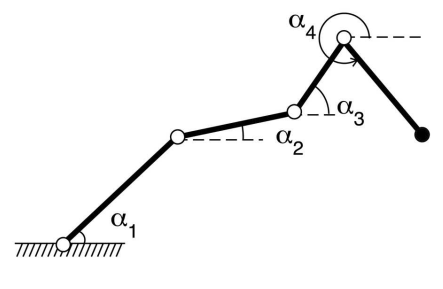
\includegraphics[scale=0.5]{images/planar-robot-arm.png}
    \caption[Planar Robot Arm]{Planar Robot Arm. (Image Source: Farber 2003)}
\end{figure}

Similarly, the configuration space of a robot arm in the $3$-dimensional space $\RR^3$ is the Cartesian product of $n$copies of the two-dimensional sphere $\Sb^2$, that is
\[
    \Sb^2 \times \Sb^2 \times \cdots \times \Sb^2
\]

\begin{thm}\cite{farber2003topological}
    Let $X  = \Sb^m \times \ldots \times \Sb^m$ be a cartesian product of $n$ copies of the $m-$-dimensional sphere $\Sb^m$. Then
    \[
        \tcomp(X) = \begin{cases}
            n + 1  & \text{if $m$ is odd}  \\
            2n + 1 & \text{if $m$ is even}
        \end{cases}
    \]
\end{thm}

\begin{proof}
    To show this result we firstly show that the LHS is less or equal to the RHS and also show otherwise too. 
    To show the first inequality we use the method of induction. 
    For the base case $n = 1$, the result holds by considering the result in theorem  (\ref{tcomp-of-sphere}).

    Now suppose the inequality is true for all $n = k$, then we have the following
    \[
        \tcomp(X) = \begin{cases}
            k + 1  & \text{if $m$ is odd}  \\
            2k + 1 & \text{if $m$ is even}
        \end{cases}
    \]
    Let $X_k$ be the cartesian product of $k$ copies of the $m$-dimensional sphere, then by the product inequality property of $\tcomp(X)$ we have
    \[
        \tcomp(X_k \times \Sb^m) \le \tcomp(X_k) + \tcomp(\Sb^m) - 1
    \]
    then we have for odd $m,\, \tcomp(X_k \times \Sb^m) \le k +2$ and for even $m,\, \tcomp(X_k \times \Sb^m) \le 2k +3$, which shows our inductive step. 
    Hence, showing the first inequality.

    Conversely, for the second inequality, let $a_i \in H^m(X, \QQ)$ denote the cohomology class which is the pull-back of the fundamental class of $\Sb^m$ under the projection $X \ra \Sb^m$ onto the $i$-th factor; for $i = 1, 2, \ldots, n$. 
    We notice that
    \[
        \prod_{i=1}^{n} (1 \otimes a_i - a_i \otimes 1) \neq 0 \in H^*(X \times X, \QQ)
    \]
    This shows that $\zdcl(X)$ is at least $n$. If $m$ is even then
    \[
        \prod_{i=1}^{n} (1 \otimes a_i - a_i \otimes 1)^2 \neq 0 \in H^*(X \times X, \QQ)
    \]
    Hence for $m$ even, $\zdcl(X)$ is at least $2n$, applying lemma \ref{zdcl:bound} completes the proof.

\end{proof}

